%% ---------------------------------------------------------------------------
%% intro.tex
%%
%% Introduction
%%
%% $Id: intro.tex 1477 2010-07-28 21:34:43Z palvarado $
%% ---------------------------------------------------------------------------

\chapter{Introducción}
\label{chp:intro}

El mejoramiento de las im\'agenes es un proceso en el que se obtiene un realce de las caracter\'isticas o informaci\'on relevante y la atenuaci\'on de informaci\'on poco importante o no deseada en una imagen. Esto permite mejorar la efectividad de m\'etodos de segmentaci\'on, rastreo de objetos, clasificaci\'on y otras t\'ecnicas de reconocimiento de patrones y el aprendizaje autom\'atico \cite{BF2014,IMPROVESEGMENTATIONBF,CONCAPAN2016}. 

Los filtros espaciales son utilizados para la reducci\'on del ruido en im\'agenes. Estos filtros act\'uan mediante la manipulaci\'on directa de los valores de los pixeles en el plano de la imagen, a diferencia de los filtros en frecuencia en los que se realiza una conversi\'on de dominio por medio de la Transformada de Fourier para realizar operaciones en el dominio de la frecuencia.

El filtro Non-Local Means (NLM) propuesto en \cite{buades2005non} se basa en el ponderamiento de la similitud entre los vecindarios de los pixeles contenidos en una ventana de búsqueda deslizante para as\'i asignar el peso correspondiente a cada pixel. Este enfoque ha demostrado resultados destacables en t\'erminos relaci\'on se\~nal-ruido y poca degradaci\'on o p\'erdida de detalles (como por ejemplo los bordes) en comparaci\'on con otros filtros como el de mediana y el bilateral \cite{CONCAPAN2016}. 

Existen mejoras desarrolladas a partir del algoritmo NLM como el propuesto en \cite{calderon2015dewaff} llamado Deceived Non-Local Means (DNLM). Presenta una combinaci\'on del m\'etodo Unsharp Masking (USM) con el filtro NLM por medio del desacoplamiento de la imagen utilizada en el pesado y la imagen usada en el filtrado. Esto permite reducir los artefactos no deseados en las im\'agenes (efecto de anillo) generados por el enfoque convencional, es decir, al aplicar primero el m\'etodo USM y posteriormente el filtro NLM \cite{calderon2015dewaff}.  

Uno de los principales inconvenientes del filtro NLM es su complejidad computacional: en el peor de los casos, para una imagen de entrada de $N$ pixeles utilizando un tamaño de ventana deslizante de $A\times B = N$ y un tamaño de vecindario de $A\times B = N$, la complejidad computacional est\'a dada por $\mathcal{O}(N^{3})$, tardando hasta $32s$ en el filtrado de una imagen de 1024x1024 pixeles \cite{Zhu2016}. Esto hace que el filtro DNLM sea poco pr\'actico para los investigadores de \'areas como la microbiolog\'ia, ya que frecuentemente necesitan analizar videos de actividad celular compuestos por cientos de miles de im\'agenes, implicando m\'ultiples d\'ias de procesamiento  \cite{Yang2006NucleiSU, cellsegmentationMarkov, Tay2010, Fils_BfilCells_2008}. De ah\'i que no es suficiente implementar las optimizaciones algor\'itmicas, sino que debe acompa\~narse con una adecuada estrategia de paralelizaci\'on y vectorizaci\'on para el mayor aprovechamiento de los recursos.

Una forma de reducir la complejidad computacional del filtro es mediante el uso de optimizaciones o aproximaciones del algoritmo. Este proyecto pretende continuar el trabajo realizado previamente, que consisti\'o en el desarrollo de una propuesta de optimizaci\'on para el filtro DNLM por medio del uso de Im\'agenes Integrales y la Transformada R\'apida de Fourier (DNLM-IIFFT). Esta optimizaci\'on permite reducir la complejidad del algoritmo a  $\mathcal{O}(N^{2}\log(N))$. Los resultados experimentales arrojan una aceleraci\'on de hasta 10 veces en el procesamiento de una imagen de 1280x720 pixeles. Si bien estos resultados presentan una aceleraci\'on considerable, es necesario explorar t\'ecnicas de paralelizaci\'on que permitan una mayor reducci\'on del tiempo de ejecuci\'on del algoritmo. 

La estrategia de paralelizaci\'on propuesta en este trabajo se enfoca en la paralelizaci\'on del algoritmo a nivel intra-nodo, para el aprovechamiento total de los n\'ucleos de procesamiento y unidades vectoriales presentes en la arquitectura. Para lograrlo, se emplea la biblioteca Intel Integrated Primitives (Intel IPP) utilizando datos alineados en memoria para una eficiente vectorizaci\'on y el uso de OpenMP para la paralelizaci\'on a nivel de hilos en el proceso de filtrado. Este esquema de paralelizaci\'on intra-nodo se escala a m\'ultiples nodos de procesamiento como se muestra en la figura \ref{fig:diagram1}.


\begin{figure}[H]
  \centering
  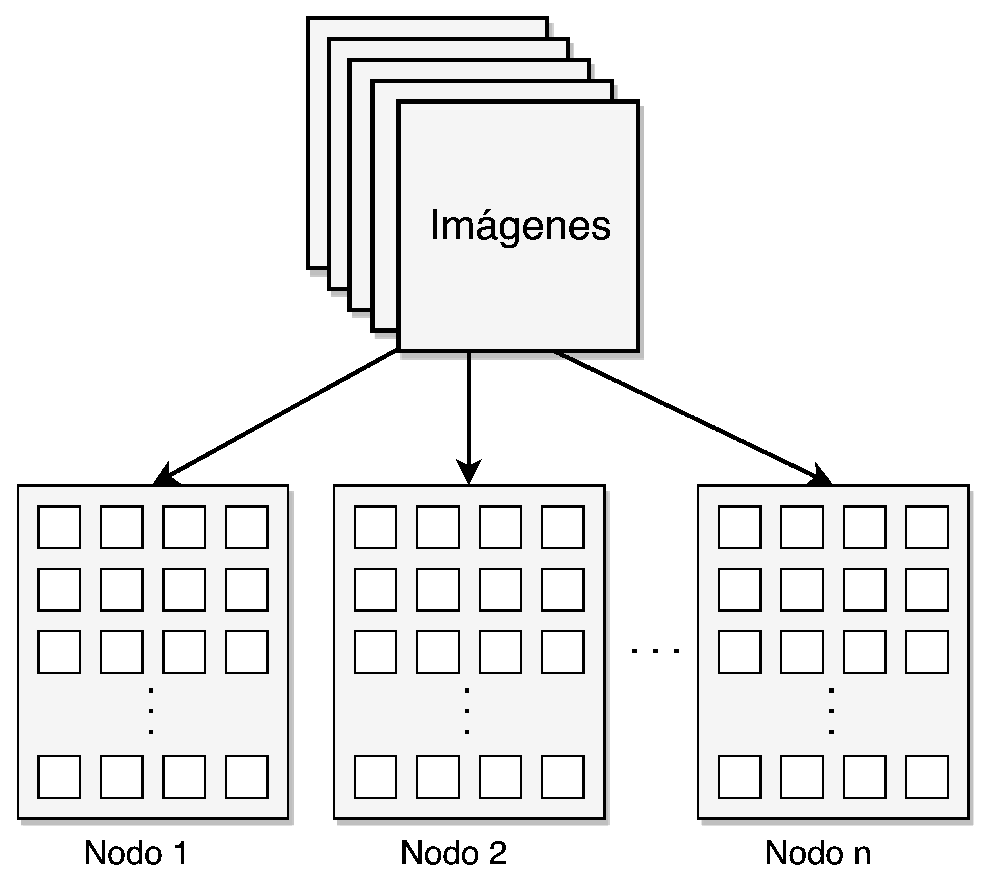
\includegraphics[width=0.9\textwidth]{blockD}
  \caption{Diagrama de bloques de la soluci\'on}
  \label{fig:diagram1}
\end{figure}

Este trabajo forma parte del proyecto de investigaci\'on llamado "Análisis funcional genómico de células cancerosas por RNA de interferencia para la identificación de redes de regulación asociadas a proliferación y muerte en respuesta a quimioterapia genotóxica", financiado por el Fondo Especial para la Educaci\'on Superior (FEES).


\section{Objetivos y estructura del documento}

\index{objetivos}

Este trabajo tiene como objetivo la paralelizaci\'on del filtro DNLM-IIFFT optimizado para la arquitectura Xeon Phi Knights Landing, para el procesamiento de conjuntos de im\'agenes. La paralelizaci\'on se realiza en varios niveles: paralelismo a nivel de tareas y paralelismo a nivel del datos. El paralelismo a nivel de tareas se emplea en el procesamiento del conjunto de im\'agenes mediante la asignaci\'on del filtrado de una imagen a cada uno de los nodos del c\'uster. Bajo este mismo principio, se emplea la distribuci\'on del procesamiento de la imagen en bloques de filas para cada uno de los hilos en el nodo de computaci\'on, con el objetivo de explotar la localidad de cach\'e. El paralelismo a nivel de datos se emplea en la vectorizaci\'on de operaciones, mediante el uso de datos alineados en memoria y la biblioteca Intel IPP. Finalmente se realiza una evaluaci\'on de la soluci\'on propuesta por medio de una comparaci\'on entre las optimizaciones y la versi\'on original del filtro DNLM.


\index{estructura}
La presente tesis est\'a organizada de la siguiente manera: el cap\'itulo \ref{chp:intro} corresponde a la introducci\'on, el contexto en el que se desarrolla este trabajo y los objetivos. Seguidamente en el cap\'itulo 2 se detalla el marco te\'orico necesario para el desarrollo de la tesis y en el cap\'itulo 3 se presenta la soluci\'on. El cap\'itulo 4 corresponde al desarrollo del experimento y finalmente, se presentan las conclusiones y el trabajo futuro en el cap\'itulo 5. 


%Esta plantilla LaTeX tiene como objetivo simplificar la construcción del
%documento de tesis, presentando ejemplo de figuras y tablas, así como otorgar
%una plataforma de compilación en GNU/Linux que simplifique la administración de
%todo el documento.
%
%La última sección de la introducción usualmente sí tiene un título estandar que
%es ``Objetivos y estructura del documento'', donde se presentan \emph{en prosa}
%los objetivos general y específicos que ha tenido el proyecto de tesis,
%así como la estructura de la tesis (por ejemplo, ``en el siguiente capítulo se
%esbozan los fundamentos teóricos necesarios para explicar en el
%capítulo~\ref{ch:solucion} la propuesta realizada$\ldots$''

%%% Local Variables: 
%%% mode: latex
%%% TeX-master: "main"
%%% End: 
